\documentclass[11pt,aspectratio=169]{beamer}
\usepackage[T1]{fontenc}
\usepackage{lmodern}
\usepackage{tikz}
\usepackage{array}
\newcolumntype{P}[1]{>{\raggedright\arraybackslash}p{#1}}

\definecolor{Ink}{HTML}{20344F}
\definecolor{Teal}{HTML}{008A99}
\definecolor{Muted}{HTML}{697E8D}
\definecolor{Pale}{HTML}{F2F5F7}
\setbeamercolor{normal text}{fg=Ink,bg=white}
\setbeamercolor{frametitle}{fg=Ink}
\setbeamercolor{title}{fg=Ink}
\setbeamercolor{structure}{fg=Teal}
\setbeamerfont{title}{size=\LARGE,series=\bfseries}
\setbeamerfont{frametitle}{size=\Large,series=\bfseries}
\setbeamertemplate{navigation symbols}{}
\setbeamertemplate{footline}{\hfill\textcolor{Muted}{\scriptsize\insertframenumber}\hspace{5mm}\vspace{3mm}}
\setbeamersize{text margin left=8mm,text margin right=8mm}
\setbeamertemplate{frametitle}{\vspace{3mm}\insertframetitle\par}
\setlength{\parskip}{5pt}
\newcommand{\planrow}[2]{\textcolor{Teal}{\textbf{#1}} & #2 \\\noalign{\vskip 12pt}}
\newcommand{\milestonerow}[3]{\textcolor{Teal}{\textbf{#1}} & \textcolor{Teal}{\textbf{#2}} & #3 \\\noalign{\vskip 12pt}}
\title{Micro-Robot Swarm}
\subtitle{Project plan}
\author{}
\date{}

% Sources: docs/planning/MILESTONES.md and AGENTS.md.
% The roadmap describes planned capability, not verified completion.
\begin{document}

\begin{frame}[plain]
\vspace{8mm}
{\LARGE\bfseries Micro-Robot Swarm\par}
\vspace{4mm}
{\Large\textcolor{Teal}{Project plan}\par}
\vspace{9mm}
M1--M5 delivery and planned expansion through M8
\vspace{7mm}

\textcolor{Muted}{Desktop supervision of ESP32-C6 robots\\using external visual feedback}
\end{frame}

\begin{frame}{Project objective and system scope}
\textbf{An operator draws a route. A robot follows it using camera feedback.}
\vspace{4mm}

\begin{tabular}{@{}P{3.1cm}P{10.7cm}@{}}
\planrow{Desktop application}{Camera acquisition, calibrated localization, planning and supervisory motion control}
\planrow{Robot firmware}{Motor regulation, command watchdog and local safe stop on each ESP32-C6}
\end{tabular}
\vspace{3mm}

\small\textcolor{Muted}{C++20 / Qt 6 / OpenCV\quad BLE commands\\macOS development and early Linux support}
\end{frame}

% Architecture follows AGENTS.md and the milestone roadmap.
\begin{frame}{Application architecture}
\small
\begin{tabular}{@{}P{3.1cm}P{10.7cm}@{}}
\planrow{Camera and vision}{Timestamped frames feed AprilTag detection and calibration. Live cameras and recorded video share one interface.}
\planrow{Tracking and world}{The tracker filters observations and marks stale poses. One authoritative WorldModel holds metric robot state.}
\planrow{Planning and control}{Tasks produce paths and motion references. Supervisory control compares desired motion with fresh visual feedback.}
\planrow{Robot communication}{RobotManager owns connections. A transport interface isolates BLE from planning and control.}
\end{tabular}

\textcolor{Muted}{The GUI observes services and accepts operator commands. Worker services keep camera and control processing responsive.}
\end{frame}

\begin{frame}{M1--M5 capability plan}
\small
\begin{tabular}{@{}P{0.65cm}P{2.85cm}P{10.0cm}@{}}
\milestonerow{M1}{Foundation}{Responsive camera preview, replay/simulation and portable build/test infrastructure}
\milestonerow{M2}{Localization}{AprilTags, camera/table calibration and fresh robot poses in metres}
\milestonerow{M3}{Communication}{BLE command/telemetry, manual control and emergency stop}
\milestonerow{M4}{Point control}{Vision feedback drives one robot to a selected target with safe stop rules}
\milestonerow{M5}{Path tracking}{Mouse-drawn paths, smoothing, trajectory generation and Pure Pursuit}
\end{tabular}
\end{frame}

% Detail slides describe planned deliverables, not completion claims.
\begin{frame}{M1--M2: camera foundation and localization}
\small
\begin{tabular}{@{}P{3.1cm}P{10.7cm}@{}}
\planrow{M1: reliable input}{Select, start and stop a camera. Handle removal safely and use recorded video for repeatable development.}
\planrow{M1: core services}{Separate camera and transport adapters from the core. Add configuration, logging and hardware-free GoogleTest/CTest checks.}
\planrow{M2: calibration}{Estimate camera intrinsics and distortion. Calibrate the tabletop transform and save profiles per camera/resolution.}
\planrow{M2: robot state}{Associate AprilTags with robot IDs. Produce filtered metric poses, with timestamps and fresh/stale/lost states.}
\end{tabular}

\textcolor{Teal}{\textbf{Exit evidence: responsive video and measured position/orientation accuracy}}
\end{frame}

\begin{frame}{M3--M4: communication and feedback control}
\small
\begin{tabular}{@{}P{3.1cm}P{10.7cm}@{}}
\planrow{M3: BLE interface}{Discover and connect an ESP32-C6. Exchange versioned commands and telemetry with sequence and freshness checks.}
\planrow{M3: safe operation}{Provide manual control and emergency stop. Verify reconnect behaviour and the robot-side command watchdog.}
\planrow{M4: target control}{Select a target in world coordinates. Use a differential-drive model to generate bounded linear and angular velocity commands.}
\planrow{M4: safety states}{Pause or stop when tracking becomes stale or communication fails. Record commands and measured pose for evaluation.}
\end{tabular}

\textcolor{Muted}{M3 builds on M1. Integrated M4 control requires both M2 localization and M3 communication.}
\end{frame}

\begin{frame}{M5: operator paths and trajectory tracking}
\small
\begin{tabular}{@{}P{3.1cm}P{10.7cm}@{}}
\planrow{Operator input}{Select a robot and draw a route on the calibrated view. Store the path in metres so display resizing preserves its geometry.}
\planrow{Path preparation}{Simplify and smooth the drawn points while respecting workspace boundaries. Generate a bounded motion reference.}
\planrow{Path following}{Use Pure Pursuit as the baseline controller. Show the desired path, actual robot trace and execution progress.}
\planrow{Execution and tests}{Support pause, cancel and safe completion. Evaluate representative shapes using cross-track RMSE, maximum error and completion time.}
\end{tabular}

\textcolor{Teal}{\textbf{M5 completes the core interaction after M4 point control is validated}}
\end{frame}

% Source: docs/archive/GITHUB_PROJECT_GANTT.md, snapshot 2026-10-10.
% Original chart end dates are exclusive. Labels below use inclusive deadlines.
% Bars describe remaining-work spans, not full milestone duration or completion.
% Later Linux issues are outside this archived schedule.
\begin{frame}{M1--M5 Gantt chart}
{\small\textcolor{Muted}{Recorded planning baseline: 12 October--28 November 2026}}
\vspace{2mm}

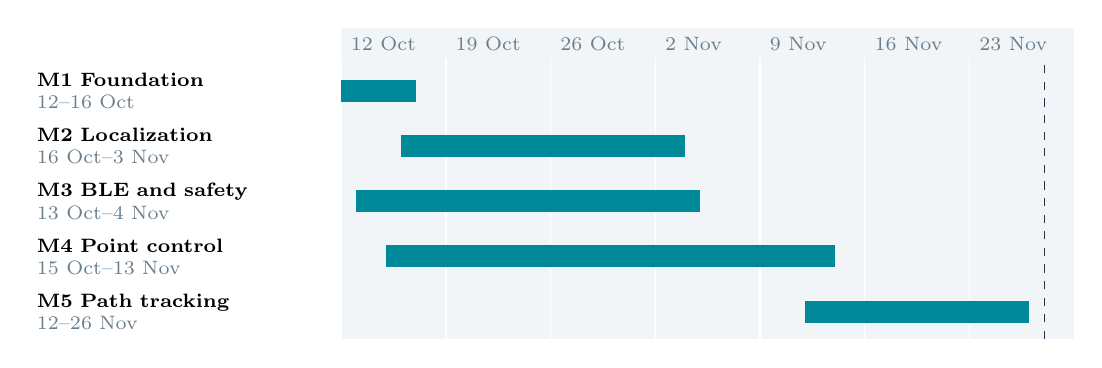
\begin{tikzpicture}[x=0.19cm,y=0.70cm]
  \fill[Pale] (0,0.5) rectangle (49,6.15);
  \foreach \x/\label in {0/12 Oct,7/19 Oct,14/26 Oct,21/2 Nov,28/9 Nov,35/16 Nov,42/23 Nov} {
    \draw[white,line width=0.5pt] (\x,0.5)--(\x,5.6);
    \node[anchor=west,font=\scriptsize,text=Muted] at (\x,5.85) {\label};
  }
  \foreach \y/\name/\dates/\start/\finish in {
    5/{M1 Foundation}/{12--16 Oct}/0/5,
    4/{M2 Localization}/{16 Oct--3 Nov}/4/23,
    3/{M3 BLE and safety}/{13 Oct--4 Nov}/1/24,
    2/{M4 Point control}/{15 Oct--13 Nov}/3/33,
    1/{M5 Path tracking}/{12--26 Nov}/31/46
  } {
    \node[anchor=east,align=left,text width=3.55cm,font=\scriptsize] at (-1,\y) {\textbf{\name}\\\textcolor{Muted}{\dates}};
    \fill[Teal] (\start,\y-0.20) rectangle (\finish,\y+0.20);
  }
  % Offset 47 is 28 November, the hard target date.
  \draw[Ink,dashed] (47,0.5)--(47,5.6);
\end{tikzpicture}

\textcolor{Teal}{\textbf{Target: 28 November 2026}}

{\tiny\textcolor{Muted}{Baseline snapshot: 10 Oct 2026. Later Linux additions require schedule review. Bars show plans.}}
\end{frame}

% M6--M8 have no assigned dates in the source roadmap.
% M7 requires M5, with M6 strongly recommended.
% Windows support remains planned until build and hardware verification.
\begin{frame}{Planned expansion through M8}
\small
\begin{tabular}{@{}P{0.65cm}P{2.85cm}P{10.0cm}@{}}
\milestonerow{M6}{Autonomous paths}{Manual obstacles, occupancy grid, footprint inflation and A* for one robot}
\milestonerow{M7}{Coordination}{Concurrent robot tasks, conflict prediction and prioritized or reservation planning}
\milestonerow{M8}{Portability}{Windows build/deployment and device verification, with adapters that preserve the core}
\end{tabular}

\textcolor{Muted}{Optional extensions: Zigbee, second-camera fusion, onboard Wi-Fi video, LiDAR and task allocation}
\vspace{2mm}

\textcolor{Teal}{\textbf{Expansion dates remain to be planned after core validation}}
\end{frame}

\begin{frame}{Validation and project completion}
\textbf{M1--M5 plus quantitative evaluation form the minimum thesis system}
\vspace{4mm}

\small
\begin{tabular}{@{}P{3.1cm}P{10.7cm}@{}}
\planrow{Capability checks}{Demonstrate calibrated tracking, BLE control and repeatable path execution}
\planrow{Safety checks}{Verify stale-pose stop, lost-connection response, watchdog and emergency stop}
\planrow{Thesis evidence}{Report localization error, latency, path RMSE/max error and completion time}
\end{tabular}
\end{frame}

\end{document}
